\section{Návrh riešenia}
\subsection{Špecifikácia požiadaviek}
V tejto sekcii sa oboznámime s požiadavkami, ktoré má naša aplikácia spĺňať. Rozdelíme ich na funkcionálne a nefunkcionálne požiadavky. Taktiež si predstavíme diagram prípadov použitia a sekvenčné diagramy niektorých procesov.
\subsubsection{Funkcionálne požiadavky}
Funkcionálne požiadavky určujú, čo presne je možné v aplikácii robiť, alebo akú má funkcionalitu.\\
\textbf{Zoznam funkcionálnych požiadaviek}
\begin{itemize}
    \item \textbf{registrácia} - používateľ sa môže zaregistrovať pomocou používateľského mena a hesla
    \item \textbf{prihlásenie} - používateľ sa môže prihlásiť pomocou používateľského mena a hesla
    \item \textbf{odhlásenie} - používateľ sa môže z aplikácie odhlásiť
    \item \textbf{nahranie trás} - používateľ môže do aplikácie nahrať ZIP súbor obsahujúci trasy
    \item \textbf{zobrazenie nahraných trás} - používateľ môže zobraziť zoznam všetkých súborov, ktoré nahral a boli úspešne spracované aplikáciou
    \item \textbf{zobrazenie všetkých trás v nahranom súbore} - používateľ môže na mape zobraziť trasy, ktoré nahral v ZIP súbore
    \item \textbf{zobrazenie jednotlivých trás v nahranom súbore} - používateľ môže na mape zobraziť jednodlivo trasy, ktoré obsahuje ZIP súbor, ktorý nahral
    \item \textbf{pripnutie trás k cestnej sieti} - používateľ môže zobraziť trasy spracované aplikáciou, ktoré sú pripnuté k cesnej sieti. Zobraziť môže všetky trasy, ktoré obsahuje ZIP súbor, ktorý nahral, alebo jednotlivo.
    \item \textbf{zobrazenie chybových nahraných súborov} - v prípade, že nahraný súbor nemal správny formát alebo bola jeho štruktúra nevhodná, sa tento súbor uloží na neskoršie stiahnutie a používateľ je informovaný o chybe, ktorá nastala
    \item \textbf{znovu-spustenie chybných súborov} - v prípade, že sa nejaké trasy nachádzajú v priečinku chybových súborov, je možné na týchto trasách znova spustiť algoritmus pripnutia trás k cestnej sieti. Ide o špeciálny prípad použitia, keď si používateľ nahrá na server súbory bez toho, aby ich dával do ZIP súboru. Týmto sa ušetrí čas pri komprimovaní trás do ZIP súboru a pri rozbaľovaní ZIP súboru.
\end{itemize}
\subsubsection{Nefunkcionálne požiadavky}
Nefunkcionálne požiadavky sa týkajú toho, ako má systém pracovať. Popisujú parametre systému a nie to, čo má systém robiť.\\
\textbf{Zoznam nefunkcionálnych požiadaviek}
\begin{itemize}
    \item \textbf{jednoduchosť a prehľadnosť} - aplikácia má byť jednoduchá na použitie a po prečítaní návodu na použitie má byť jasné ako má byť použitá
    \item \textbf{prehľadný kód} - kód má byť písaný prehľadne, aby sa v budúcnosti dal jednoducho rozšíriť a aby bol udržateľný
    \item \textbf{jasná informácia o chybnej trase} - ak nastane chyba pri nahraní alebo spracovaní trás, používateľ má byť jasne informovaný, kde nastala chyba
\end{itemize}
\subsubsection{Diagramy}
\begin{figure}[H]
    \centering
    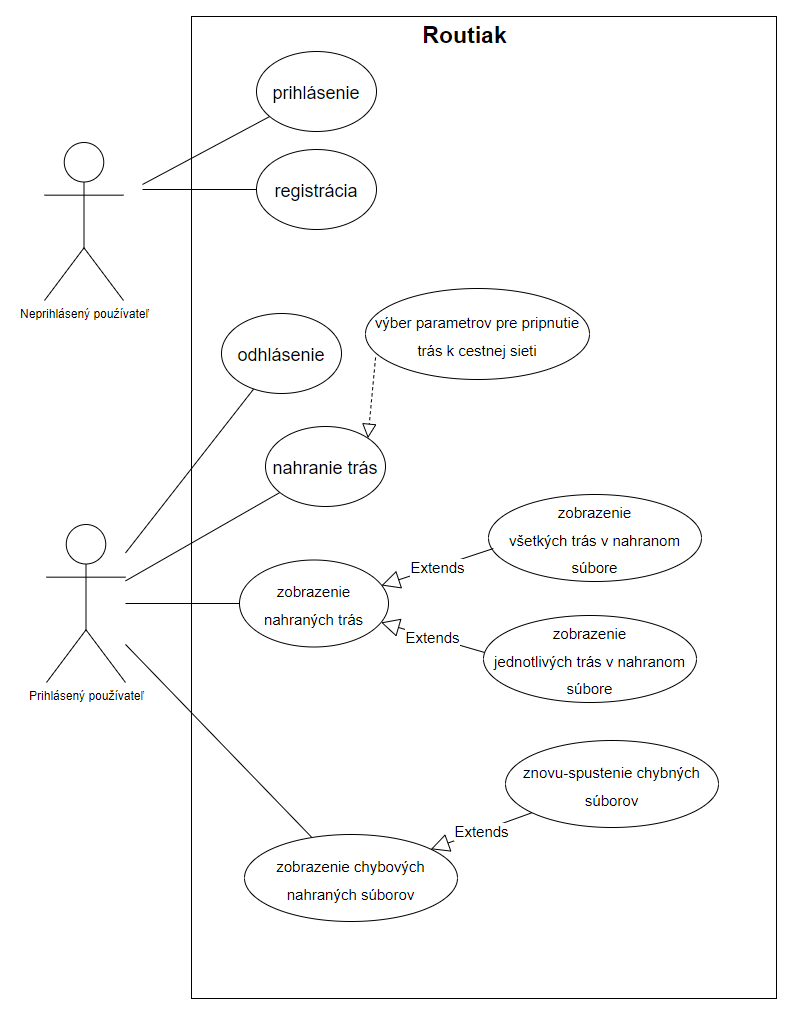
\includegraphics[width=0.7\textwidth]{img/diagramy/use-case.png}
    \caption{Diagram prípadov použitia}
    \label{fig:use-case}
\end{figure}
Používateľ sa bude musiet po otvorení webovej aplikácie prihlásiť alebo registrovať. Po prihlásení sa roľa pouźívateľa zmení na prihláseného. Ako prihlásený bude používateľ môcť nahrať trasy vo formáte ZIP. Pri nahrávaní súboru musí taktiež zvoliť parametre, ktoré budú použité systémom pri pripínaní trás k cestnej sieti. Prihlásený používateľ si bude môcť zobraziť trasy rozdelené podľa súborov, ktoré nahral. Trasy v týchto súboroch bude potom môcť zobraziť všetky naraz, alebo jednotlivo. Taktiež si bude môcť zobraziť chybové nahrané súbory v prípade, že nejaké chybové súbory nahral. Na týchto chybových súboroch bude potom môcť spustiť algoritmus pripínania trás k cestnej sieti znova. Nižšie je možné vidieť priebeh procesov nahrania súborov (obr.\ref{fig:seq-upload-zip}), zobrazenia trás (obr.\ref{fig:seq-show-routes}) alebo zobrazenia chybových súborov (obr. \ref{fig:seq-show-errors}) pomocou sekvenčných diagramov.
\begin{figure}[H]
    \centering
    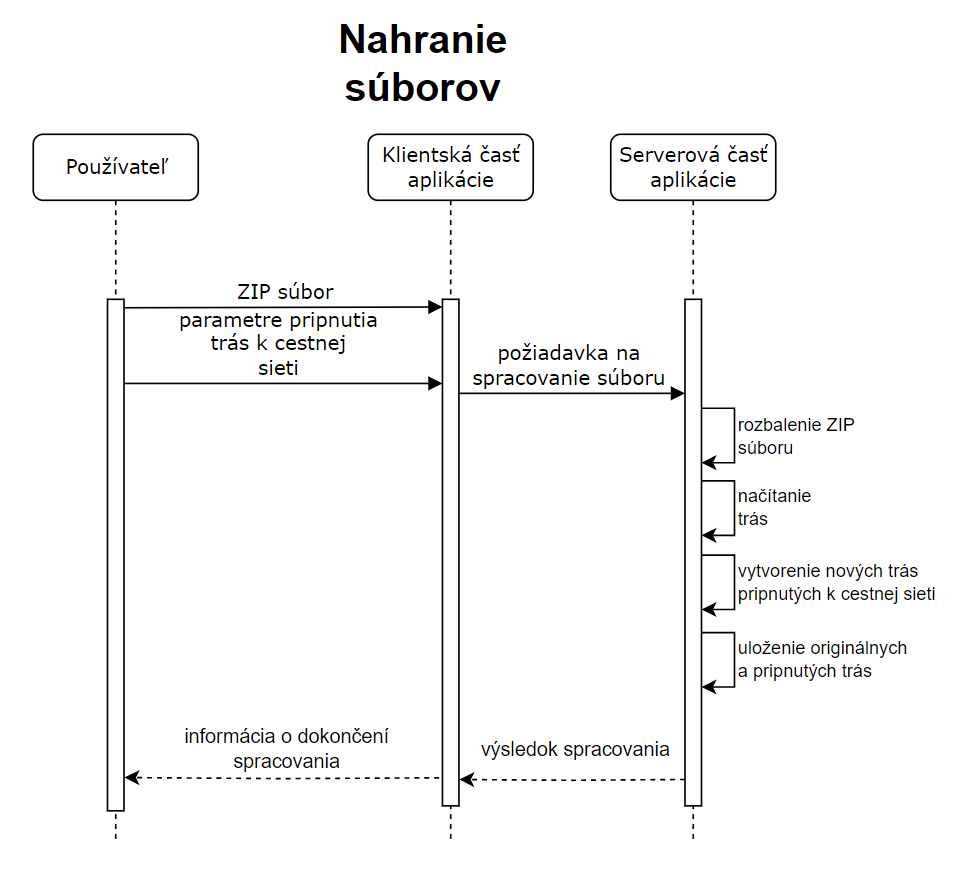
\includegraphics[width=0.7\textwidth]{img/diagramy/sekvencny-nahranie.png}
    \caption{Sekvenčný diagram procesu nahrania súborov na server.}
    \label{fig:seq-upload-zip}
\end{figure}
\begin{figure}[H]
    \centering
    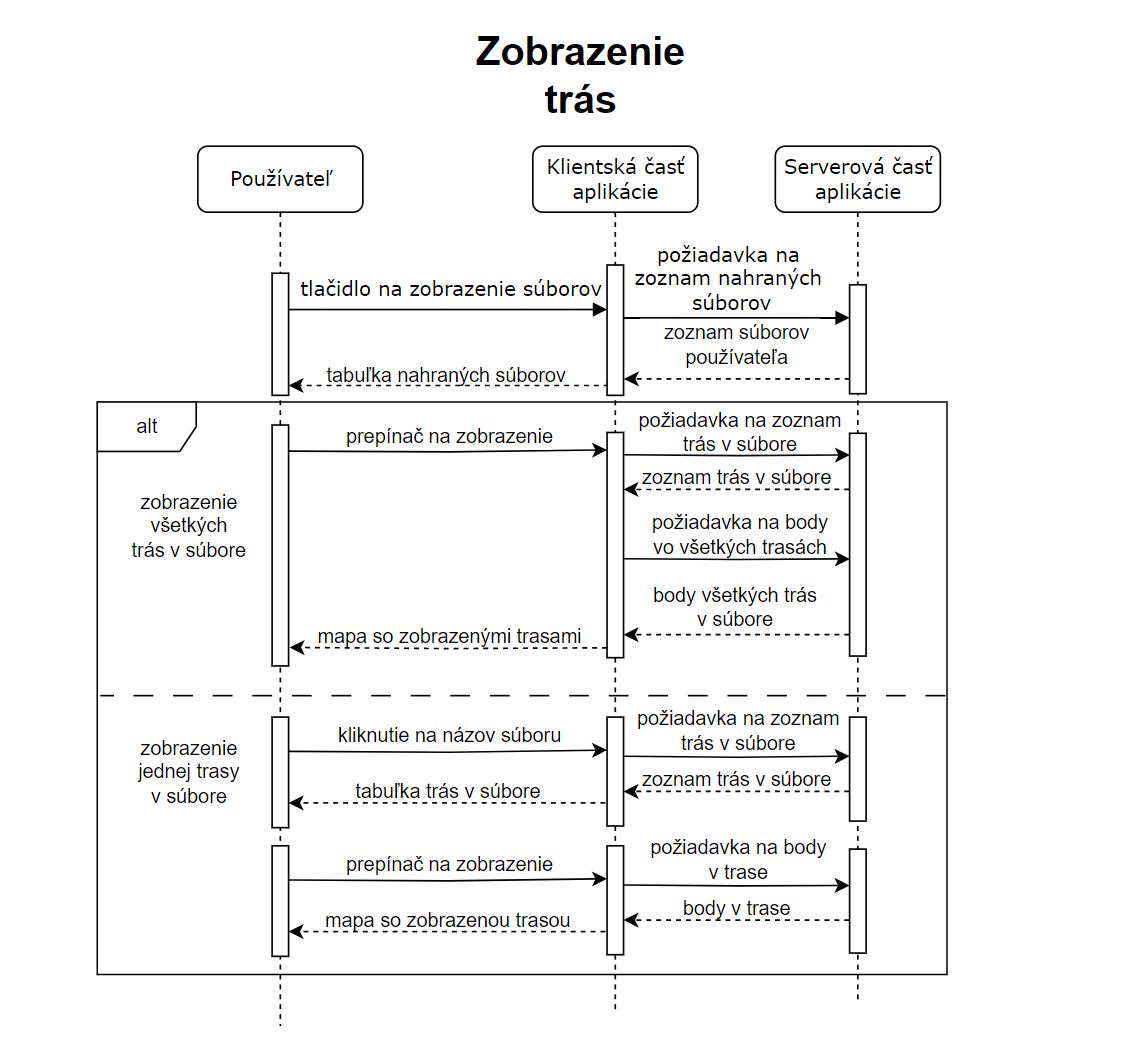
\includegraphics[width=0.7\textwidth]{img/diagramy/sekvencny-trasy.png}
    \caption{Sekvenčný diagram procesu zobrazenia trás na mape.}
    \label{fig:seq-show-routes}
\end{figure}
\begin{figure}[H]
    \centering
    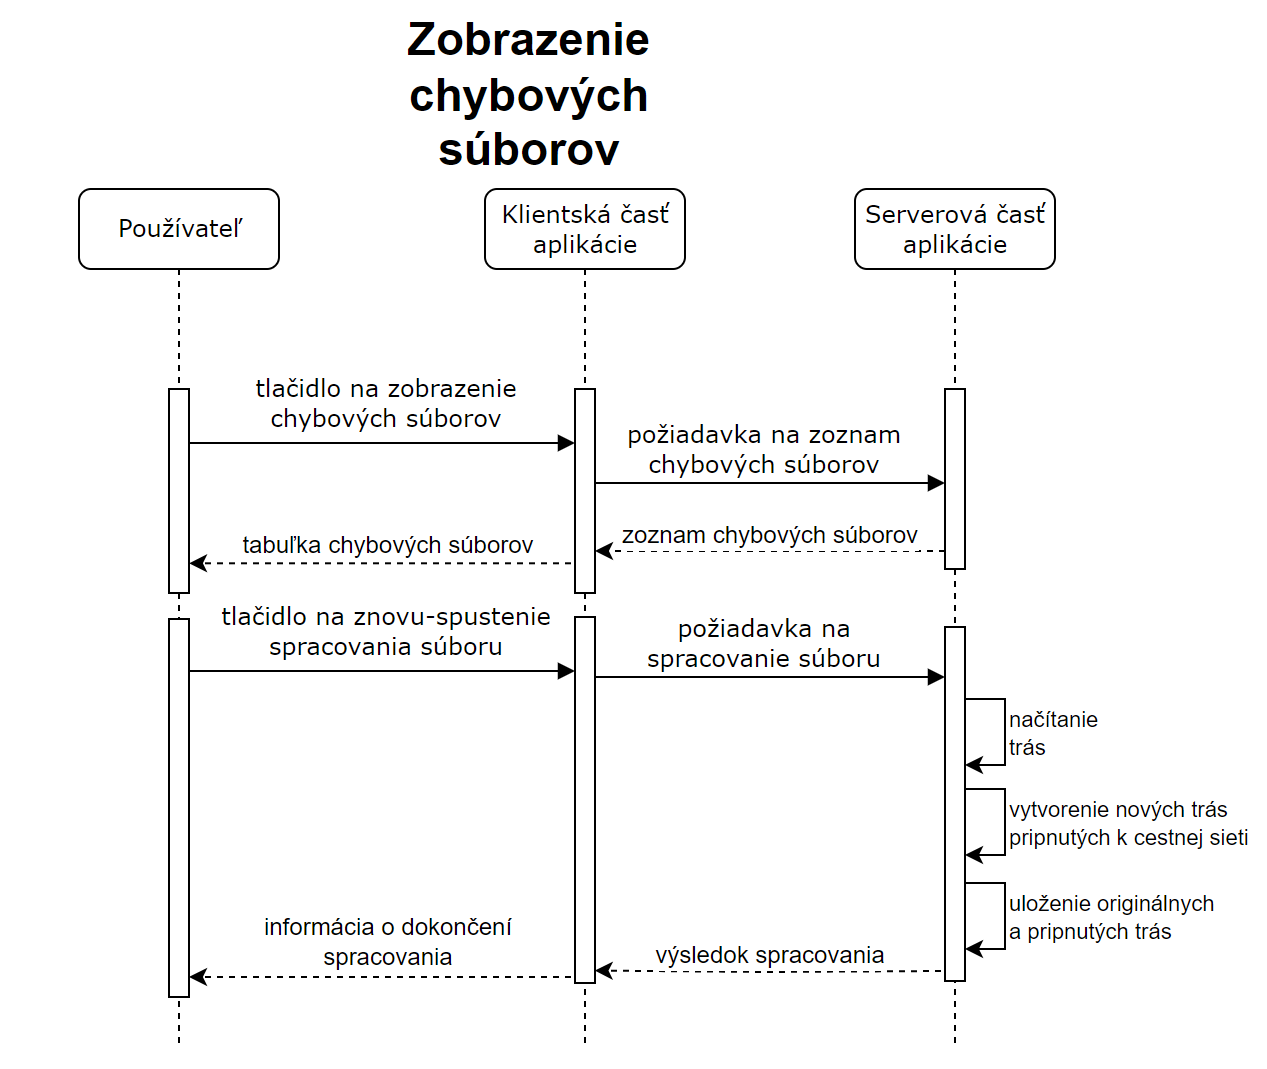
\includegraphics[width=0.7\textwidth]{img/diagramy/sekvencny-chybove.png}
    \caption{Sekvenčný diagram procesu zobrazenia chybových súborov}
    \label{fig:seq-show-errors}
\end{figure}

\subsection{Ukladanie údajov}
V aplikácii sú vytvorené priečinky \textit{uploads} a \textit{routes}. Do priečinka \textit{uploads} sa budú ukladať všetky nahrané súbory. Po nahratí ZIP súboru na server bude pre používateľa vytvorený priečinok, ktorého názov bude zodpovedať prihlasovaciemu menu používateľa. V priečinku používateľa sa vytvorí nový priečinok \textit{unzipped}, v ktorom sa vytvorí priečinok s názvom nahraného ZIP súboru. Do tohto priečinku sa rozbalí nahraný ZIP súbor. Cesta k tomuto priečinku sa uloží do premennej, s ktorou algoritmus neskôr bude pracovať. Po skončení algoritmu prebehne kontrola, ktorá určí či boli všetky trasy v ZIP súbore spracované správne. V prípade, že v ZIP súbore bude nejaká chybová trasa, ZIP súbor spolu s rozbalenými súbormi ostane na serveri pre neskoršie stiahnutie používateľom alebo prípadné znovu-spustenie algoritmu. V opačnom prípade sa priečinok aj s nahraným ZIP súborom vymaže, aby sa ušetrilo miesto na serveri.

Štruktúra priečinka \textit{routes} bude podobná priečinku \textit{uploads}. Do priečinka \textit{routes} sa po dokončení algoritmu vytvorí priečinok (ak ešte neexistuje), ktorého názov bude zodpovedať prihlasovaciemu menu používateľa. V priečinku používateľa bude vytvorený priečinok s názvom zodpovedajúcim názvu nahraného ZIP súboru. Do priečinku s názvom súboru budú vytvorené priečinky, ktorých názov bude zodpovedať názvom trás, ktoré boli nahrané v ZIP súbore a ktoré boli úspešne spracované algoritmom pripínania trás k cestnej sieti. V každom takomto priečinku budú dva súbory s názvom \textit{original.csv} a \textit{map-match.csv}, ktoré budú obsahovať konkrétne body trasy. 

Štuktúry priečinkov sú vizualizované na obrázkoch . Priečinky sú zobrazené zaobleným obdĺžnikom a súbory sú zobrazené obdĺžnikom. Tri bodky \textit{"..."} vertikálne medzi priečinkami a súbormi symbolizujú, že v priečinku môže byť 0 až N súborov. To znamená, že môže byť priečinok prázdny, alebo v ňom môže byť ľubovoľný počet súborov/priečinkov. Tri bodky \textit{"..."} horizontálne za priečinkom symbolizujú, že graf pokračuje ale pre zjednodušenie obrázka bol graf skrátený.

\begin{figure}[H]
    \centering
    \begin{subfigure}{\textwidth}
      \centering
      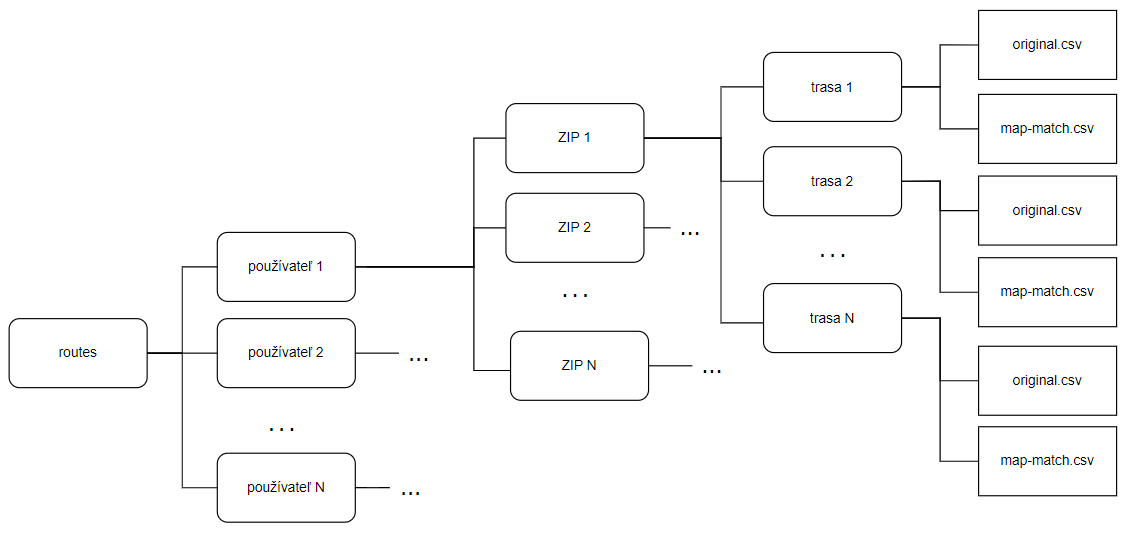
\includegraphics[width=1\textwidth]{img/struktura priecinkov/routes.png}
      \caption{Štruktúra priečinku \textit{routes}}
      \label{fig:routes-structure}
    \end{subfigure}
    \begin{subfigure}{\textwidth}
      \centering
      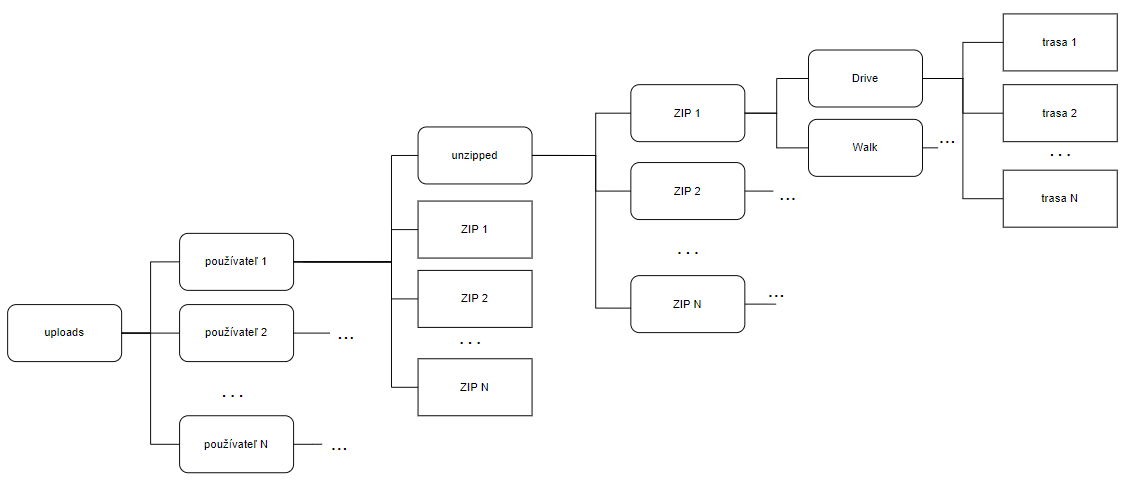
\includegraphics[width=1\textwidth]{img/struktura priecinkov/uploads.png}
      \caption{Štruktúra priečinku \textit{uploads}}
      \label{fig:uploads-structure}
    \end{subfigure}
    \caption{Štruktúry priečinkov \textit{uploads} a \textit{routes}.}
    \label{fig:uploads-routes-structure}
  \end{figure}


\subsection{Spôsoby pripínania trás k cestnej sieti}
\subsubsection{Routing}
\subsubsection{Map matching}